\section{Mathematical programming}

We can divide mathematical programs in:
\begin{itemize}
    \item Linear Programming (LP)
    \item Semi-Definite Programming (SDP)
\end{itemize}

A mathematical program contains:
\begin{itemize}
    \item varibles $x_1, \dots, x_n$ ($x_i \in \mathbb{R}$ or $x_i \in \mathbb{Q}$)
    \item objective function $f(x_1, \dots, x_n)$ (either to minimize or to maximize)
    \item constraint functions $g_i(x_1, \dots, x_n) \leq b_i$ (or $g_i(x_1, \dots, x_n) \geq b_i$), for $i = 1, \dots, n$
\end{itemize}

In a linear program, the objective function $f$ is linear and each constraint function $g_i$ is linear as well.

When we force each variable to be an integer, the progam is called \textbf{Integer Program}.

\begin{definition}[Feasible solution]
    A solution is said to be feasible if it satisfied all constraints.
\end{definition}

\subsection{Some examples}

    \begin{equation}
        \begin{cases}
            \max x_1 + x_2\\
            x_1 \geq 3\\
            x_2 \geq 5\\
            x_1 \leq 2.5
        \end{cases}
    \end{equation}

    This program clearly has no solutions, since the constraints $x_1 \geq 3$ and $x_1 \leq 2.5$ can't be both satisfies ad the same time.

    \begin{equation}
        \begin{cases}
            \max x_1 + x_2\\
            x_2 \geq 5\\
            x_1 \leq 2.5
        \end{cases}
    \end{equation}

    There are infinitely many solutions, and the "optimal value" of this LP is unbounded ($\infty$).

    \begin{equation}
        \begin{cases}
            \max x_1 + x_2\\
            2 x_1 + x_2 \leq 10\\
            x_1 \geq 0
            x_2 \geq 0
        \end{cases}
    \end{equation}

    We can set $x_1 = 0$ and $x_2 = 10$. All the constraints are satisfied and our objective function would have value $10$.


\subsection{Hardness of LPs}
    If $f(x_1, \dots, x_n) = \sum_{j=1}^n c_j x_j$ and $g_i(x_1, \dots, x_n) = \sum_{j=1}^n a_{ij} x_j$, then if each coefficient $c_j$ and $a_{ij}$ and each term $b_i$ is a rational number, representable with at most $t$ bits, then the LP can be optimized in time $O(n \cdot m \cdot t)^c$, for come constant $c > 0$.

    IPs are instead harder to solve than LPs. In general, we can't solve an IP in polynomial time.
    What can be done, and will be done later for some problems, is to give an IP program for a problem, that will be tranformed into an LP, easier to solve.



\subsection{Solution for Vertex Cover}\label{subsec:vc_lp}

    We now see a pratical use of LPs to solve the Vertex Cover problem.

    Let our set of variables be $\{ x_v \st v \in V \}$. We define our IP, for a graph $G(V,E)$ to be the following:
    \begin{equation}\label{eq:lp_vc}
        \begin{cases}
            \min \sum_{v \in V} x_v\\
            x_u + x_v \geq 1    & \forall \{ u,v \} \in E\\
            x_v \in \B          & \forall v \in V
        \end{cases}
    \end{equation}

    Solving this IP would give us an optimal VC.

    Let $x_{v_1}^*, x_{v_2}^*, \dots, x_{v_n}^*$ be an optimal solution to the IP. Define $S^* = \{ v \st v \in V \wedge x_v^* = 1 \}$.

    \begin{theorem}
        $S^*$ is an optimal VC of $G(V,E)$.
    \end{theorem}

    \begin{lemma}
        $S^*$ is a vertex cover.
    \end{lemma}

    \begin{proof}
        $S^*$ being a VC means that $\forall \{u,v\} \in E$, $u \in S^*$ or $v \in S^*$ or both (i.e. $u,v \in S^*$).
        Given that $x_u^* + x_v^* \geq 1$, $\forall \{ u,v \} \in E$, and that $x_u^*, x_v^* \in \B$, at least one of $x_u^*$ and $x_v^*$ is equal to $1$.
        Thus $u \in S^*$ or $v \in S^*$.
    \end{proof}

    \begin{lemma}
        If $S$ is a VC, then there exists a feasible solution $\{ x_v \}_{v \in V}$ to the IP, s.t. $\sum_{v \in V} x_v = \cardinality{S}$.
    \end{lemma}

    \begin{proof}
        $x_v = 1 \leftrightarrow v \in S$.
    \end{proof}

    \begin{corollary}
        An optimal solution to the IP has value equal to
        \[ \min_{\substack{S \subseteq V\\ S \text{ is a VC}}} \cardinality{S} \]
    \end{corollary}

    Recall that IPs can't be solve, in general, in polytime, while LPs can.
    So we \textit{relax} the IP for VC (see equation \ref{eq:lp_vc}) into an LP.
    
    \begin{equation}\label{eq:ip_vc}
        \begin{cases}
            \min \sum_{v \in V} x_v\\
            x_u + x_v \geq 1    & \forall \{ u,v \} \in E\\
            0 \leq x_v \leq 1   & \forall v \in V
        \end{cases}
    \end{equation}

    Note the the two programs are almost the same, except that, during the relaxation, we've allowed each variable from being in $\B$, to being in the range $[0,1]$.
    Albeit this is not how IPs are always transformed into LPs, it is indeed quite often the case, and it is the way in which most (if not all) of the IPs during this course will be transformed into LPs.

    It is easy transforming the IP into a VC solution: for a vertex $v$, $x_v = 1$ iff $v$ is in the vertex cover.
    In the LP we have fractional values, so how do we choose vertices? We apply a \textbf{rounding rule}: an algorithm that, given an LP solution, outputs a VC set.

    The rounding rule for this problem is quite simple.
    We define 
    \[ S = \{ v \st x_v \geq \frac{1}{2} \wedge v \in V \} \]

    \begin{lemma}
        $S$ is a vertex cover.
    \end{lemma}

    \begin{proof}
        Let $\{ u,v \} \in E$. The LP contains the constraint $x_u + x_v \geq 1$.
        Given that our solution guarantees that $x_u + x_v \geq 1$ (the LP solution is feasible by definition),
        $x_u + x_v \geq 1 \rightarrow \max (x_u, x_v) \geq \frac{x_u + x_v}{2} \geq \frac{1}{2}$.

        Thus, $u \in S$, or $v \in S$ (or both), thus the edge $\{ u,v \}$ is covered.
    \end{proof}

    \begin{lemma}\label{lemma:lp_vc1}
        $\cardinality{S} \leq 2 \sum_{v \in V} x_v$.
    \end{lemma}

    \begin{proof}
        $\cardinality{S} = \sum_{v \in S} 1 \overset{(v \in S \rightarrow x_v \geq \frac{1}{2})}{\leq} \sum_{v \in S} 2 x_v = 2 \sum_{v \in S} x_v \overset{(x_v \geq 0)}{\leq} 2 \sum_{v \in V} x_v$
    \end{proof}

    Recall that the LP minimizes $\sum_{v \in V} x_v$. Let $\{ x_v^* \}_{v \in V}$ be an optimal solution to the LP.
    Let $S^*$ be the result of the application of our rounding rule; i.e. $S^* = \{ v \st v \in V \wedge x_v^* \geq \frac{1}{2} \}$.
    \[ \cardinality{S^*} \overset{(\text{Lemma } \ref{lemma:lp_vc1})}{\leq} 2 \sum_{v \in V} x_v^* = 2 LP^* \overset{(\text{LP relaxation of IP})}{\leq} 2 IP^* = 2 \min_{\substack{S \subseteq V\\ S \text{ is a VC}}} \cardinality{S} = 2 OPT \]

    If Lemma~\ref{lemma:lp_vc1} could be improved (to, say, $\cardinality{S} \leq 1.9 \sum_{v \in V} x_v$), then the approximation ration would be directly improved.

    Let us define the \textbf{integrality gap} to be the ratio between the optimal IP solution and the optimal LP solution. That is,
    \[ IG = \frac{IP^*}{LP^* } \]

    Now, let us consider a particular graph s.t. we can use it show an upper bound on the integrality gap.
    This approach will be used also in the future: build a special instance of a problem, s.t. the instance can be used to show lower or upper bound to the optimality of approximations.

    Consider the graph $G(V,E) = K_3$ (i.e.~the complete graph with $3$ vertices).

    \begin{lemma}
        Each optimal solution for $G(V,E)$ contains two nodes.
    \end{lemma}

    \begin{lemma}
        $x_1 = x_2 = x_3 = \frac{1}{2}$ is a feasible solution of value $\frac{3}{2}$.
    \end{lemma}

    \begin{proof}
        $\forall \{ i,j \} \in E$, $x_i + x_j = 2 \frac{1}{2} = 1 \geq 1$. Thus each constraint is satisfied.

        The objective value is $3 \frac{1}{2} = \frac{3}{2}$.
    \end{proof}

    \begin{lemma}
        There exists no feasible LP solution of value $< \frac{3}{2}$.
    \end{lemma}

    \begin{proof}
        For $\{ i,j \} \in E$, $x_i + x_j \geq 1$.

        $2 \sum_{v \in V} x_v = 2 x_1 + 2 x_2 + 2 x_3 = (x_1 + x_2) + (x_2 + x_3) + (x_1 + x_3) \overset{\text{feasibility}}{\geq} 1 + 1 + 1 = 3 $.

        Thus $\sum_{v \in V} \geq \frac{3}{2}$.
    \end{proof}

    \begin{corollary}
        $LP^* = \frac{3}{2}$ and $IP^* = 2$.
    \end{corollary}

    Thus, for $K_3$, $IG = \frac{IP^*}{LP^*} = \frac{2}{\frac{3}{2}} = \frac{4}{3}$. So $IG \leq 2$.

    \begin{exercise}
        Show that $\forall \varepsilon > 0$, $\exists G(V,E)$ s.t. $\dfrac{OPT_{VC}(G(V,E))}{LP^*(G(V,E))} \geq 2 - \varepsilon$.

        Hints:
        \begin{itemize}
            \item $K_t$, large $t$
            \item Prove the optimal VC for $K_t$ has $t-1$ nodes
            \item What is the optimal LP solution for $K_t$?
        \end{itemize}
    \end{exercise}


\subsection{Set Cover problem} \label{subsect:setcover}

    Input: $U = [n] = \{ 1, \dots, n \}$, $S_1, \dots, S_m \subseteq U$.

    We call the input $U$, meaning our \textit{universe} set.

    Question: what is the size of a smallest class of subsets $T \subseteq [m]$ s.t. $\bigcup_{j \in T} S_j = U$?

    Let us see an example. Let $U = [4] = \{ 1,2,3,4 \}$, and let $S_1 = \{ 1,2 \}$, $S_2 = \{ 2,3 \}$, $S_3 = \{ 3,4 \}$.
    A solution, even optimal, is $S_1 \cup S_3 = [4]$.

    Set Cover (SC) is NP-Hard. We consider an LP solution to approximate it. We first see an IP problem, translated into an LP.

    Let the IP be
    \begin{equation}
        \begin{cases}
            \min \sum_{j=1}^m x_j                               & (x_j = 1 \text{ if } S_j \text{ is in the solution})\\
            \sum_{j \in [m] \text{ s.t. } i \in S_j} x_j \geq 1 & \forall i \in [n]\\
            x_j \in \B                                          & \forall j \in [m]
        \end{cases}
    \end{equation}

    The LP relaxation is
    \begin{equation}
        \begin{cases}
            \min \sum_{j=1}^m x_j                               \\
            \sum_{j \in [m] \text{ s.t. } i \in S_j} x_j \geq 1 & \forall i \in [n]\\
            0 \leq x_j \leq 1                                   & \forall j \in [m]
        \end{cases}
    \end{equation}

    The constraint $\sum_{j \in [m] \text{ s.t. } i \in S_j} x_j \geq 1$ means that each element of $[n]$ has to be picked at least once.

    \begin{observation}
        $LP^* \leq IP^*$
    \end{observation}

    \begin{proof}
        The LP is a relaxation to the IP (the constraint of the LP are less stringent than those of the IP).
        Thus each IP solution is also an LP solution.
    \end{proof}

    We now need a rounding rule, to converto the LP solution into a solution for Set Cover.
    This rounding rule is a randomized procedure, less trivial than the one used for VC. Many rouding rules are actually randomized, like this one.

    \begin{algorithm}
    \caption{Randomized rounding technique}\label{alg:rand_round_sc}
    \begin{algorithmic}%[1]
        \State~$A \gets \emptyset$
        \State~let $x^*$ be an optimal LP solution
        \For{$k=1$ to $\lceil 2 \ln{n} \rceil$}
            \For{$j = 1$ to $m$}
                \State~flip an independent coin with head probability $x_j^*$
                \If{the coin is heads}
                    \State~$A \gets A \cup \{ S_j \}$
                \EndIf
            \EndFor
        \EndFor
    \end{algorithmic}
\end{algorithm}

    The first for loop is a repetition of "phases". It represents how many times do we want to repeat the subprocedure in the second loop, the one that loops over sets and adds them to the solution.

    As it is going to be clearer later on, since this procedure is randomized, it is not always the case that the output $A$ is indeed a set cover.
    
    The number of times we repeat the first loop actually defines a sort of trade off.
    The more times we repeat it, the higher the probability that $A$ is a set cover, but also the higher the probability that we put too many sets in the solution, leading to a solution worse than the optimal.
    
    \begin{lemma}
        Consider a generic iteration $k$ of the outer loop.
        Let $p_i$ be the probability in iteration $k$ that at least on of the sets containing $i$ gets added to $A$.
        Then $p_i \geq 1 - \frac{1}{e} \approx 0.633\dots$.
    \end{lemma}

    \begin{proof}
        To prove this lemma we are going to use that fact that $1 - x \leq e^{-x}$.

        $\prob[i \text{ not covered in iteration } k] = \prod_{j \in [m] \text{:} i \in S_j} (1 - x_j^*) \leq \prod_{j \in [m] \text{:} i \in S_j} e^{-x_j^*} = e^{- \sum_{j \in [m] : i \in S_j}} \overset{\text{(feasibility of solution)}}{\leq} e^{-1}$.

        Thus $\prob[i \text{ covered in iteration } k] \geq 1 - \frac{1}{e}$.
    \end{proof}

    \begin{lemma}\label{lemma:sc_2}
        Pick $i \in [n]$. $\prob[i \text{ not covered by any set in } A] \leq \frac{1}{n^2}$.
    \end{lemma}

    \begin{proof}
        $\prob[i \text{ not covered by any set in } A] = \prod_{k=1}^{\lceil 2 \ln n \rceil} \prob[i \text{ not covered in iteration } k] \leq \prod_{k=1}^{\lceil 2 \ln n \rceil} \frac{1}{e} = e^{- \lceil 2 \ln n \rceil} = n^{-2} $ 
    \end{proof}

    \begin{lemma}
        $\prob[A \text{ is a set cover}] \geq 1 - \frac{1}{n}$
    \end{lemma}

    \begin{proof}
        $\prob[A \text{ is not a set cover}] \overset{\text{(UB)}}{\leq} \sum_{i=1}^n \prob[i \text{ not covered by } A] \overset{\text{(Lemma \ref{lemma:sc_2})}}{\leq} \sum_{i=1}^{n} \frac{1}{n^2} = \frac{n}{n^2} = \frac{1}{n}$
    \end{proof}

    \begin{lemma}
        $\expected[\cardinality{A}] \leq \lceil 2 \ln n \rceil LP^* \leq \lceil 2 \ln n \rceil OPT_{SC}$
    \end{lemma}

    \begin{proof}
        Fix an iteration $k$ of the outer loop. Let $A_k$ be the class of sets added to $A$ in iteration $k$.

        $\expected[\cardinality{A_k}] \overset{(\text{linearity of } \expected)}{=} \sum_{i=1}^{m} x_j^* = LP^* \leq OPT_{SC}$

        $A = A_1 \cup A_2 \cup \dots \cup A_k \cup \dots \cup A_{\lceil 2 \ln n \rceil}$.
        
        $\cardinality{A} \leq \sum_{i = 1}^{\lceil 2 \ln n \rceil} \cardinality{A_i}$. Then $\expected[\cardinality{A}] \leq \sum_{i=1}^{\lceil 2 \ln n \rceil} \expected[\cardinality{A}] = \sum_{i=1}^{\lceil 2 \ln n \rceil} LP^* \leq \lceil 2 \ln n \rceil LP^* \leq \lceil 2 \ln n \rceil OPT_{SC}$.
    \end{proof}

    So, let us consider the following statement
    \[ ? \overset{\exists \text{ instance}}{\leq} \frac{OPT_{SC}}{LP_{SC}^*} \overset{\forall \text{ instance}}{\leq} \lceil 2 \ln n \rceil \]

    If we manage to find an instance with an IG smaller than $\frac{OPT_{SC}}{LP_{SC}^*}$, then we have proved a lower bound on the integrality gap of set cover.
    
    We know of such an instance, that we shall see in a moment. As it is the case, the following will be proved
    \[ \dfrac{1}{4 \ln 2} \ln n \overset{\exists \text{ instance}}{\leq} \frac{OPT_{SC}}{LP_{SC}^*} \overset{\forall \text{ instance}}{\leq} \lceil 2 \ln n \rceil \]

    An improvement, albeit a small one.

    Let us consider the following universe set, $E = \{ e_A \st A \in \binom{[q]}{\frac{q}{2}}, \text{ for some even } q \geq 2 \}$.

    For $n = \cardinality{E} = \binom{q}{\frac{q}{2}} = \Theta(\frac{2^q}{\sqrt{q}}) \Rightarrow q \geq \log n - \Theta(\log \log n)$.

    $\forall i \in [q]$, let us define $S_i = \{ e_A \st e_A \in E \wedge i \in A \}$ and $C = \{ S_i \st i \in [q] \}$. $\cardinality{C} = q \overset{\Delta}{=} m$.

    Let us see an example. Given $q = 4$:
    \begin{itemize}
        \item $E = \{ e_{12}, e_{13}, e_{14}, e_{23}, e_{24}, e_{34} \}$
        \item $S_1 = \{ e_{12}, e_{13}, e_{14} \}$
        \item $S_2 = \{ e_{12}, e_{23}, e_{24} \}$
        \item $S_3 = \{ e_{13}, e_{23}, e_{34} \}$
        \item $S_4 = \{ e_{14}, e_{24}, e_{34} \}$
    \end{itemize}

    \begin{lemma}
        $LP_{SC}^* \leq 2$
    \end{lemma}

    \begin{proof}
        Consider the LP solution $_1 = x_2 = \cdots = x_q = \frac{2}{q}$, with $q = n$.
        This solution has value $\sum_{i=1}^{q} x_i = q \frac{2}{q} = 2$.

        The generic LP constraint is $\sum_{s_j : e_a \in S_j} x_j \geq 1$, $\forall e_a \in E$.

        $\sum_{s_j : e_a \in S_j} x_j = \sum_{s_j : e_a \in S_j} \frac{2}{q} = \cardinality{A} \frac{2}{q} = \frac{q}{2} \frac{2}{q} = 1 \geq 1$. Thus the solution is feasible.
    \end{proof}

    \begin{lemma}
        $OPT_{SC} \geq \frac{1}{2} \log_2 n - O(\log \log n)$
    \end{lemma}

    \begin{proof}
        Assume by contradiction that the sets $S_{i_1}, S_{i_2}, \dots, S_{i_k}$, for $k \leq \frac{q}{2}$, cover each element of the instance.
        Consider also the set $T = [q] \setminus \{ i_1, \dots, i_k \}$.
        Then $\exists A \subseteq T$ s.t. $\cardinality{A} = \frac{q}{2}$ (because $\cardinality{T} \geq q - k \geq \frac{q}{2}$), then $e_A \in E$.

        The element $e_A$ is not covered by $S_{i_1}, S_{i_2}, \dots, S_{i_k}$, because $A \cap \{ i_1, \dots, i_k \} = \emptyset$.
        Then $S_{i_1}, S_{i_2}, \dots, S_{i_k}$ is not a set cover if $k \leq \frac{q}{2}$.

        It follows that the minimum set cover contains $\geq \frac{q}{2} + 1$ sets.
    \end{proof}

    Thus $IG = \dfrac{OPT_{SC}}{LP_{SC}^*} \overset{(\text{on some instances})}{\geq} \dfrac{\frac{1}{2} \log_2 n - O(\log \log n)}{2} \approx \frac{1}{4} \log_2 n$


\subsection{Densest subgraph problem}\label{subsec:densestsubgraph_problem}

    Input: $G(V,E)$

    Question: what is the subset $S \subseteq V$ having maximum \textbf{density}?

    We define density as follows:
    \[ \rho(S) = \dfrac{\cardinality{E(S)}}{\cardinality{S}} \]
    Where $E(S) = \{ \{u,v\} \st \{u,v\} \in E \wedge u,v \in S \}$.

    A variation of the problem is the following.
    For $k$-densest subgraph we want $S \subseteq V$, $\cardinality{S} = k$, s.t. $\cardinality{E(S)}$ is as large as possible.

    To solve this problem, we give an LP program.
    \begin{equation}\label{eq:densestsubgraph_lp}
        \begin{cases}
            \max \sum_{\{i,j\} \in E} x_{\{i,j\}}                           \\
            x_{\{i,j\}} \leq y_i                    & \forall \{i,j\} \in E \\
            x_{\{i,j\}} \leq y_j                    & \forall \{i,j\} \in E \\
            \sum_{i \in V} y_i \leq 1                                       \\
            x_{\{i,j\}} \geq 0                      & \forall \{i,j\} \in E \\
            y_i \geq 0                              & \forall i \in V
        \end{cases}
    \end{equation}

    \begin{lemma}\label{lemma:densestsubgraph_1}
        For any $G(V,E)$, $\forall S \subseteq V$, $\exists$ feasible solution to the LP, having value $\geq \frac{\cardinality{E(S)}}{\cardinality{S}} = \rho(S)$.
    \end{lemma}

    \begin{proof}
        For $i \in S$, set $y_i = \frac{1}{\cardinality{S}}$.
        For $i \in V \setminus S$, set $y_i = 0$.
        For each $\{i,j\} \in E$, set
        \begin{equation}
            x_{\{i,j\}} = 
            \begin{cases}
                \frac{1}{\cardinality{S}} & \text{if } \{i,j\} \in E(S)\\
                0                           & \text{o/w}
            \end{cases}
        \end{equation}

        The constraint $\sum_{i \in V} y_i \leq 1$ is satisfied, given that
        $\sum_{i \in V} y_i = \sum_{i \in S} y_i + \sum_{i \in V \setminus S} y_i = \sum_{i \in S} \frac{1}{\cardinality{S}} + \sum_{i \in V \setminus S} 0 = \frac{\cardinality{S}}{\cardinality{S}} = 1$.

        Take any $\{i,j\} \in E(S)$. We have $x_{\{i,j\}} = \frac{1}{\cardinality{S}}$.
        But, if $\{i,j\} \in E(S)$, then $i,j \in S$. Thus $y_i = y_j = \frac{1}{\cardinality{S}}$.
        Then, $\forall \{i,j\} \in E(S)$, the constraints $x_{\{i,j\}} \leq y_i$ and $x_{\{i,j\}} \leq y_j$ are both satisfied.

        If instead $\{i,j\} \not\in E(S)$, then $x_{\{i,j\}} = 0$.
        Thus $x_{\{i,j\}} \leq y_i$ and $x_{\{i,j\}} \leq y_j$ are both satisfied by $y_i, y_j \geq 0$.

        Thus, our solution is feasible.

        The value of the solution is:
        \[ \sum_{\{i,j\} \in E} x_{\{i,j\}} = \sum_{\{i,j\} \in E(S)} x_{\{i,j\}} = \sum_{\{i,j\} \in E(S)} \frac{1}{\cardinality{S}} = \dfrac{\cardinality{E(S)}}{\cardinality{S}} = \rho(S) \]
    \end{proof}

    \begin{lemma}\label{lemma:densestsubgraph_2}
        For any feasible LP solution of value $v$, $\exists S \subseteq V$ s.t. $\rho(S) \geq v$.
    \end{lemma}

    \begin{proof}
        Let $Y', X'$ be a feasible LP solution of value $v$.
        Let $Y, X$ be the solution to the LP s.t.
        \begin{itemize}
            \item $y_i = y_i'$, $\forall i \in V$
            \item $x_{\{i,j\}} = \min(y_i,y_j)$, $\forall \{i,j\} \in E$
        \end{itemize}

        The $Y,X$ solution is feasible, indeed:
        \begin{itemize}
            \item $\sum_{i \in V} y_i = \sum_{i \in V} y_i' \leq 1$
            \item $\forall \{i,j\} \in E$, it holds $x_{\{i,j\}} \leq y_i$ and $x_{\{i,j\}} \leq y_j$
        \end{itemize}

        We have to provide a set $S$ having density at least $v$.
        We are going to provide a number of $S$'s, one of which will have the desired property.
        $\forall r \geq 0$, let us consider
        \[ S(r) = \{ i \st y_i \geq r \} \]
        \[ E(r) = \{ \{i,j\} \st x_{\{i,j\}} \geq r \} \]

        We can observe that $\{i,j\} \in E(r) \leftrightarrow i \in S(r)$ and $j \in S(r)$.
        The proof is left as an exercise.

        We claim that $\exists r \geq 0$ s.t. $\rho(S(r)) = \dfrac{\cardinality{E(r)}}{\cardinality{S(r)}} \geq \sum_{\{i,j\} \in E} x_{\{i,j\}} = v$.

        Proof of claim. We define a permutation $\pi$ of the nodes s.t.
        \[ 0 \leq y_{\pi(1)} \leq y_{\pi(2)} \leq \cdots \leq y_{\pi(n-1)} \leq y_{\pi(n)} \leq 1 \]

        %$ \int_0^1 \cardinality{E(r)} dr =
        %\int_{0}^{y_{\pi(1)}} \cardinality{S(r)}dr + \int_{y_{\pi(1)}}^{y_{\pi(2)}} \cardinality{S(r)}dr + \cdots + \int_{y_{\pi(n)}}^{1} \cardinality{S(r)}dr =
        %\int_{0}^{y_{\pi(1)}} n \; dr + \int_{y_{\pi(1)}}^{y_{\pi(2)}} (n-1)dr + \cdots + \int_{y_{\pi(n-1)}}^{y_{\pi(n)}} 1 dr + \int_{y_{\pi(n)}}^{1} 0 dr = 
        %(y_{\pi(1)} - 0)n + (y_{\pi(2)} - y_{\pi(1)})(n-1) + \cdots + (y_{\pi(n)} - y_{\pi(n-1)})1 + 0 = 
        %y_{\pi(1)} (n - (n-1)) + y_{\pi(2)}((n-1) - (n-2)) + \cdots + y_{\pi(n)}(1-0) = 
        %\sum_{i=1}^{n} y_{\pi(i)} = \sum_{i=1}^{n} y_i \leq 1$.

        \begin{equation*}
            \begin{split}
                \int_0^1 \cardinality{S(r)} dr &=\\
                    &= \int_{0}^{y_{\pi(1)}} \cardinality{S(r)}dr + \int_{y_{\pi(1)}}^{y_{\pi(2)}} \cardinality{S(r)}dr + \cdots + \int_{y_{\pi(n)}}^{1} \cardinality{S(r)}dr =\\
                    &= \int_{0}^{y_{\pi(1)}} n \; dr + \int_{y_{\pi(1)}}^{y_{\pi(2)}} (n-1)dr + \cdots + \int_{y_{\pi(n-1)}}^{y_{\pi(n)}} 1 dr + \int_{y_{\pi(n)}}^{1} 0 dr =\\
                    &= (y_{\pi(1)} - 0)n + (y_{\pi(2)} - y_{\pi(1)})(n-1) + \cdots + (y_{\pi(n)} - y_{\pi(n-1)})1 + 0 =\\
                    &= y_{\pi(1)} (n - (n-1)) + y_{\pi(2)}((n-1) - (n-2)) + \cdots + y_{\pi(n)}(1-0) =\\
                    &= \sum_{i=1}^{n} y_{\pi(i)} = \sum_{i=1}^{n} y_i \leq 1
            \end{split}
        \end{equation*}

        $  \int_0^1 \cardinality{E(r)} dr = \sum_{\{i,j\} \in E} x_{\{i,j\}} = \sum_{\{i,j\} \in E} \min(y_i, y_j) = \sum_{\{i,j\} \in E} \min(y_i', y_j') \geq \sum_{\{i,j\} \in E} x_{\{i,j\}}' = v $

        Then, $\int_0^1 \cardinality{S(r)}dr \leq 1$ and $\int_0^1 \cardinality{E(r)}dr \geq v$.

        By contradiction, supopose that $\forall r \geq 0$, $\dfrac{\cardinality{E(r)}}{\cardinality{S(r)}} < v$.
        Then $\cardinality{E(r)} < v \cardinality{S(r)}$, $\forall r \geq 0$.
        Thus $v \leq \sum_{\{i,j\} \in E} x_{\{i,j\}} = \int_0^1 \cardinality{E(r)}dr < \int_0^1 v \cardinality{S(r)} dr = v \int_0^1 \cardinality{S(r)} dr \leq v \cdot 1 = v$.

        Since $v \not< v$, we have a contradiction.
        Thus $\exists r \geq 0$ s.t. $\cardinality{E(r)} \geq v \cardinality{S(r)} \rightarrow \rho(S(r)) \geq v$.
    \end{proof}

    Thus, we can get an optimal (densest) subgraph (one of $S(y_1), \dots, S(y_n)$ will do).
    We can solve the LP in polytime, and we can transform the LP solution in an optimal subgraph.
    Is this fast enough? No, the LP has $\geq \cardinality{E}$ variables.

    \begin{corollary}
        $LP^* = OPT_{DS}$
    \end{corollary}

    \begin{proof}
        By Lemma~\ref{lemma:densestsubgraph_1}, $LP^* \geq OPT_{DS}$.
        By Lemma~\ref{lemma:densestsubgraph_2}, $LP^* \leq OPT_{DS}$.
    \end{proof}

    The LP for Densest Subgraph has $\Theta(n^2)$ variables, so albeit being polynomially solvable, the number of variables is not linear.
    For $n$ very large (e.g. $10^8 \dots 10^9$ nodes), $n^2$ is too slow.

    We now see a greedy algorithm, due to M. Charikar, to approximate Densest Subgraph.

    \begin{algorithm}
    \caption{Charikar algorithm}\label{alg:charikar_greedy}
    \begin{algorithmic}%[1]
        \Procedure{Greedy}{$G(V,E)$}
            \State~$S \gets V$
                \For{$i = 1, 2, \dots, n$}
                    \State~let $v_i$ be a node having minimum degree in $G[S_{i-1}]$
                    \State~$S_i \gets S_{i-1} \setminus \{v_i\}$
                \EndFor
                
            \Return~a set $S_i$ having larget density $\rho(S_i)$
        \EndProcedure
    \end{algorithmic}
\end{algorithm}

    \begin{exercise}
        Prove that Greedy does not always return an optimal solution.

        Hint: construct a graph s.t.~the algorithm returns a non optimal solution.
    \end{exercise}

    \begin{definition}[Orientation]
        An orientation $\phi$ of the edges of an undirected graph $G(V,E)$ is a function that assigns to each $e \in E$ one of its endpoints
        \[ \phi : E \rightarrow V \]
    \end{definition}
    
    Note that $\phi(e) \in e$.

    \begin{definition}
        Given an orientation $\phi$ of $G(V,E)$, let $d_\phi(v)$ be the in-degree of $v \in V$, according to $\phi$.
    \end{definition}

    \begin{observation}
        If $\phi$ is an orientation of $G(V,E)$, then $\sum_{v \in V} d_\phi(v) = \cardinality{E}$.
    \end{observation}

    \begin{definition}
        The max-degree of $\phi$ is $\Delta_\phi = \max_{v \in V} d_\phi(v)$.
    \end{definition}

    \begin{lemma}
        $\max_{\emptyset \subset S \subseteq V} \rho(S) = \max_{\emptyset \subset S \subseteq V} \dfrac{\cardinality{E(S)}}{\cardinality{S}} \leq \Delta_\phi$, $\forall \phi$.
    \end{lemma}

    \begin{proof}
        Let $\emptyset \subset S \subseteq V$ be given.
        Each $\{u,v\} \in E(S)$ is going to be oriented towards on of its endpoints; that is, towards a node of $S$.
        So $\cardinality{E(S)} \leq \sum_{v \in S} d_\phi(v) \leq \sum_{v \in S} \Delta_\phi = \cardinality{S} \Delta\phi$.

        Thus, $\dfrac{\cardinality{E(S)}}{\cardinality{S}} \leq \Delta_\phi$.
    \end{proof}

    While running the greedy algorithms, we \textit{build} an orientation.
    Whenever node $v_i$ (the $i^{th}$ node to be removed) is removed from the graph (which, at that point, has node set $S_{i-1}$) we orient each edge of $G[S_{i-1}]$ that is incident on $v_i$ towards $v_i$.
    The resulting orientation is called $\phi_{GR}$.

    Observe that, with orientation $\phi_{GR}$, $d_{\phi_{GR}}(v)$ equals the degree of $v$ in the graph, when $v$ is about to be removed.

    \begin{lemma}
        Let $M$ be the maximum $\rho(S_i)$ value; i.e. $M = \max_{i = 0,\dots,n-1} \rho(S_i)$.
        (Note that $M$ is the value of the greedy solution).

        Then, $\Delta_{\phi_{GR}} \leq 2M$.
    \end{lemma}

    \begin{proof}
        For $i = 1, 2, \dots, n$, $v_i$ is a node of minumum degree in $G[S_{i-1}]$.
        In general, the minumum degree in a graph is not larger than the average degree of the same graph.
        Thus
        \begin{equation*}
            \begin{split}
                d_{\phi_{GR}}(v_i) &= \min_{v \in S_{i-1}} d_{S_{i-1}}(v) \leq \avg_{v \in S_{i-1}} d_{S_{i-1}}(v) =\\
                    &= \dfrac{\sum_{v \in S_{i-1}} d_{S_{i-1}}(v)}{\cardinality{S_{i-1}}} = \dfrac{2 \cardinality{E(S_{i-1})}}{\cardinality{S_{i-1}}} = 2\rho(S_{i-1})
            \end{split}
        \end{equation*}

        Then
        \[ \Delta_{\phi_{GR}} = \max_{v_i \in V} d_{\phi_{GR}}(v_i) = \max_{i=1, \dots, n} d_{\phi_{GR}}(v_i) \leq
        \max_{i=1, \dots, n} 2 \rho(S_{i-1}) = 2M \]
    \end{proof}

    \begin{corollary}
        Greedy returns a $2$-approximation to Densest Subgraph.
    \end{corollary}

    \begin{proof}
        \[ M \geq \dfrac{\Delta_{\phi_{GR}}}{2} \geq \dfrac{\max_{\emptyset \subset S \subseteq V} \rho(S)}{2} \]

        Thus the greedy solution is not worse than a $2$-approximation.
    \end{proof}


\subsection{Primal and Dual}

    We can define an LP, in general, as a \textbf{primal} in the following way:
    \begin{equation}
        \begin{cases}
            \max c_1 x_1 + c_2 x_2 + \cdots + c_n x_n\\
            (y_1) a_{11} x_1 + a_{12} x_2 + \cdots + a_{1n} x_n \leq b_1\\
            (y_2) a_{21} x_1 + a_{22} x_2 + \cdots + a_{2n} x_n \leq b_2\\
            \vdots\\
            (y_2) a_{m1} x_1 + a_{m2} x_2 + \cdots + a_{mn} x_n \leq b_m\\
            x_1, \dots, x_n \geq 0
        \end{cases}
    \end{equation}

    The \textbf{dual} of the above LP is:
    \begin{equation}
        \begin{cases}
            \min b_1 y_1 + b_2 y_2 + \cdots + b_m y_m\\
            (x_1) a_{11} y_1 + a_{21} y_2 + \cdots + a_{m1} y_m \geq c_1\\
            (x_2) a_{12} y_1 + a_{22} y_2 + \cdots + a_{m2} y_m \geq c_2\\
            \vdots\\
            (x_n) a_{1n} y_1 + a_{2n} y_2 + \cdots + a_{mn} y_m \geq c_n\\
            y_1, \dots, y_m \geq 0
        \end{cases}
    \end{equation}

    The fact that a primal is always defined as a maximization problem, and a dual as a minimization problem, is conventional.

    Now, we can also define these programs in matrix form.

    If
    \begin{equation}
        A = 
        \begin{pmatrix}
            a_{11} & a_{12} & \cdots & a_{1n}\\
            a_{21} & a_{22} & \cdots & a_{2n}\\
            \vdots\\
            a_{m1} & a_{m2} & \cdots & a_{mn}
        \end{pmatrix}
    \end{equation}

    \begin{equation}
        b = 
        \begin{pmatrix}
            b_1\\
            \vdots\\
            b_m
        \end{pmatrix}
    \end{equation}
    
    \begin{equation}
        c = 
        \begin{pmatrix}
            c_1\\
            \vdots\\
            c_n
        \end{pmatrix}
    \end{equation}

    \begin{equation}
        X = 
        \begin{pmatrix}
            x_1\\
            \vdots\\
            x_n
        \end{pmatrix}
    \end{equation}

    \begin{equation}
        Y = 
        \begin{pmatrix}
            y_1\\
            \vdots\\
            y_m
        \end{pmatrix}
    \end{equation}

    Then the \textbf{primal} is
    \begin{equation}
        \begin{cases}
            \max c^T X\\
            AX \leq b\\
            X \geq 0
        \end{cases}
    \end{equation}

    And the \textbf{dual} is
    \begin{equation}
        \begin{cases}
            \min b^T Y\\
            A^T Y \geq c\\
            Y \geq 0
        \end{cases}
    \end{equation}

    Recall that, if $N$ and $M$ are matrices, then $(N M)^T = M^T N^T$.

    \begin{theorem}[Weak Duality]
        If 
        \begin{itemize}
            \item $X$ is a feasible solution to the primal
            \item $Y$ is a feasible solution to the dual
        \end{itemize}

        Then 
        \[ Primal(C) = c^T X \leq b^T Y = Dual(Y) \]
    \end{theorem}

    \begin{proof}
        \[ c^T X = X^T c \leq X^T A^T Y = (A X)^T Y \leq b^T Y \]
    \end{proof}


    Recall \nameref{eq:densestsubgraph_lp} LP formulation.
    Let us see it as a Primal LP (in "standard form").

    \begin{equation}
        \begin{cases}
            \max \sum_{\{i,j\} \in E} x_{\{i,j\}}\\
            (y_{ij}): x_{\{i,j\}} - x_i \leq 0  & \forall \{i,j\} \in E\\
            (y_{ji}): x_{\{i,j\}} - x_j \leq 0  & \forall \{i,j\} \in E\\
            (y^*): \sum_{i \in V} x_i \leq 1\\
            x_{\{i,j\}} \geq 0                  & \forall \{i,j\} \in E\\
            x_i \geq 0                          & \forall i \in V
        \end{cases}
    \end{equation}

    Let us now consider the equivalent Dual LP.
    \begin{equation}
        \begin{cases}
            \min y^*\\
            (x_{\{i,j\}}): y_{ij} + y_{ji} \geq 1\\
            (x_i): y^* - \sum_{j : \{i,j\} \in E} y_{ij} \geq 0\\
            y^* \geq 0\\
            y_{ij}, y_{ji} \geq 0
        \end{cases}
    \end{equation}

    Our greedy 2-approximtion for DS is esentially a dual LP solution:
    set $y^* = \Delta_{\phi_{GR}}$ and
    \begin{equation}
        y_{ij} = 
        \begin{cases}
            1 & \text{if } \{i,j\} \text{ is directed towards } i \text{ in } \phi_{GR}\\
            0 & \text{o/w}
        \end{cases}
    \end{equation}

    For the $x_{\{i,j\}}$, $y_{ij} + y_{ji} \geq 1$ is satisfied, because it is either $1+0 \geq 1$ or $0+1 \geq 1$.
    For $x_i$, $y^* \geq \sum_{j : \{i,j\} \in E} y_{ij}$. $\Delta_{\phi_{GR}} = y^* \geq \sum_{j : \{i,j\} \in E} y_{ij} = deg_{\phi_{GR}}(i)$.

    Then, each constraint is satisfied by our solution, of value $\Delta_{\phi_{GR}}$.

    \[ \dfrac{\Delta_{\phi_{GR}}}{2} \leq \text{greedy solution} \leq PRIMAL^* \leq DUAL^* \leq \Delta_{\phi_{GR}} \]

    Now, recall that \nameref{subsec:vc_lp} is a \textit{minimization} problem.
    We saw its dual:
    \begin{equation}
        \begin{cases}
            \min \sum_{v \in V} x_v\\
            y_{\{u,v\}}: x_u + x_v \geq 1\\
            x_v \geq 0
        \end{cases}
    \end{equation}

    Let us now see its primal:
    \begin{equation}
        \begin{cases}
            \max \sum_{\{u,v\} \in E} y_{\{u,v\}}\\
            x_v: \sum_{u : \{u,v\} \in E} y_{\{u,v\}} \leq 1\\
            y_{\{u,v\}} \geq 0
        \end{cases}
    \end{equation}

    For all maximal matching $M \subseteq E$. For the dual, we set
    \begin{equation}
        x_u = 
        \begin{cases}
            1 & \text{if } e \in M \text{ s.t. } u \in E\\
            0 & \text{o/w}
        \end{cases}
    \end{equation}

    Is this dual solution feasible? Yes.
    By contradiction, if $x_u + x_v < 1$, for some $\{u,v\} \in E$, we could add $\{u,v\}$ to $M$. Then $M$ wouldn't be maximal.
    What's the value of the solution? It is $\sum_{v \in V} x_v = 2 \cardinality{M}$.

    Instead, for the primal, we set
    \begin{equation}
        y_{\{u,v\}} = 
        \begin{cases}
            1 & \text{if } \{u,v\} \in M\\
            0 & \text{o/w}
        \end{cases}
    \end{equation}

    In the algorithm, if there exists and edge $e$, we add both endpoints to the solution, and then we remove them from the graph.
    THe solution is feasible because $M$ is a matching.

    \[ \cardinality{M} \leq PRIMAL^* \leq DUAL^* \leq 2 \cardinality{M} \]


\subsection{Greedy algorithms for Densest Subgraph}

    Going back to \nameref{subsec:densestsubgraph_problem}, we want to improve the greedy algorithm, by parallelizing it and possibly make it so the number of iterations is reduced.

    \begin{algorithm}
    %\caption{Charikar algorithm}%\label{alg:charikar_greedy}
    \begin{algorithmic}%[1]
        \Procedure{Parallel\_Greedy}{$G(V,E)$}
            \State~$S_0 \gets V$
            \State~$i \gets 0$
                \While{$S_i \neq \emptyset$}
                    \State~$A_i \gets \{ v \st v \in S_i \wedge \deg_{S_i}(v) = \min_{u \in S_i} \deg_{S_i}(u) \} $
                    \State~$S_{i+1} \gets S_i \setminus A_i$
                    \State~$i \gets i+1$
                \EndWhile
                
            \Return~a set $S_i$ having larget density $\rho(S_i)$
        \EndProcedure
    \end{algorithmic}
\end{algorithm}

    There are instances in which this algorithm saves many iterations, as well as instances in which it doesn't save much time. Let us think for example of a graph in which each component is two vertices connected together; it is easy to see that the graph that the algorithm would stop after only 1 iteration.
    Let us now consider a path; the algorithm, at each iteration, would remove both endpoints of the path, thus requiring $\approx \frac{n}{2}$ iterations, if $n$ is the number of nodes.

    So we need a better algorithm. See the algorithm \ref{alg:greedy_avg}.

    \begin{algorithm}
    \caption{Greedy average}\label{alg:greedy_avg}
    \begin{algorithmic}%[1]
        \Procedure{Greedy\_AVG}{$G(V,E)$}
            \State~$S_0 \gets V$
            \State~$i \gets 0$
                \While{$S_i \neq \emptyset$}
                    \State~let $v_i$ be a node s.t. $\deg_{S_i}(v_i) \leq avg_{v \in S_i} \deg_{S_i}(v)$
                    \State~$S_{i+1} \gets S_i \setminus \{v_i\}$
                    \State~$i \gets i+1$
                \EndWhile
                
            \Return~a set $S_i$ having larget density $\rho(S_i)$
        \EndProcedure
    \end{algorithmic}
\end{algorithm}

    Does this solve the problem? Not really.
    Consider a path with a triangle in one endpoint. For such a graph the algorithm requires $\approx n$ iterations.

    See the alorithm \ref{alg:greedy_parallel_avg}

    \begin{algorithm}
    \caption{Greedy average}\label{alg:greedy_parallel_avg}
    \begin{algorithmic}%[1]
        \Procedure{Greedy\_AVG}{$G(V,E)$}
            \State~$S_0 \gets V$
            \State~$i \gets 0$
                \While{$S_i \neq \emptyset$}
                    \State~$A_i \gets \{ v_i \st \deg_{S_i}(v_i) \leq \avg_{v \in S_i} \deg_{S_i}(v) \}$
                    \State~$S_{i+1} \gets S_i \setminus A_i$
                    \State~$i \gets i+1$
                \EndWhile
                
            \Return~a set $S_i$ having larget density $\rho(S_i)$
        \EndProcedure
    \end{algorithmic}
\end{algorithm}

    Still no solution. A path is once once again an instance in which this algortihm doesn't save much time.
    Though this is not a bad idea per se, so why not try to take a little more than the average?

    \begin{algorithm}
    \caption{Greedy $\varepsilon$ (Bahmani, Kumar, Vassilutski, 2012)}\label{alg:greedy_epsilon}
    \begin{algorithmic}%[1]
        \Procedure{Greedy$_\varepsilon$}{$G(V,E)$}
            \State~$S_0 \gets V$
            \State~$i \gets 0$
                \While{$S_i \neq \emptyset$}
                    \State~$A_i \gets \{ v_i \st v_i \in S_i \wedge \deg_{S_i}(v_i) \leq (1+\varepsilon)avg_{v \in S_i} \deg_{S_i}(v) \}$
                    \State~$S_{i+1} \gets S_i \setminus A_i$
                    \State~$i \gets i+1$
                \EndWhile
                
            \Return~a set $S_i$ having larget density $\rho(S_i)$
        \EndProcedure
    \end{algorithmic}
\end{algorithm}

    Now we want to prove two things about this algorithm:
    \begin{itemize}
        \item $GREEDY_\varepsilon$ gives a good approximation to DS (Lemma~\ref{lemma:ds_greedy_1})
        \item $GREEDY_\varepsilon$ runs quickly (Lemma~\ref{lemma:ds_greedy_2})
    \end{itemize}

    \begin{lemma}\label{lemma:ds_greedy_1}
        $GREEDY_\varepsilon$ returns a $2(1+\varepsilon)$-approximation, $\forall \varepsilon > 0$.
    \end{lemma}

    \begin{proof}
        Let $S^* \neq \emptyset$ be an optimal solution (then, wlog, $\cardinality{S^*} \geq 2$).

        We claim that $\forall v \in S^*$, $\deg_{S^*}(v) \geq \rho(S^*) \overset{\Delta}{=} \dfrac{\cardinality{E(S^*)}}{\cardinality{S^*}}$.

        %$\rho(S^*) = \dfrac{\cardinality{E(S^*)}}{\cardinality{S^*}} \overset{(\text{by optimality of }S^*)}{\geq} \rho(S^* \setminus \{v\}) = 
        %\dfrac{\cardinality{E(S^* \setminus \{v\})}}{\cardinality{S^* \setminus \{v\}}} = 
        %\dfrac{\cardinality{E(S^*)} - \deg_{S^*}(v)}{\cardinality{S^*}-1}$

        \begin{equation*}
            \begin{split}
                \rho(S^*) &= \dfrac{\cardinality{E(S^*)}}{\cardinality{S^*}} \overset{(\text{by optimality of }S^*)}{\geq} \rho(S^* \setminus \{v\}) =\\
                    &= \dfrac{\cardinality{E(S^* \setminus \{v\})}}{\cardinality{S^* \setminus \{v\}}} = \dfrac{\cardinality{E(S^*)} - \deg_{S^*}(v)}{\cardinality{S^*}-1}
            \end{split}
        \end{equation*}

        So $\dfrac{\cardinality{E(S^*)} - \deg_{S^*}(v)}{\cardinality{S^*}-1} \leq \dfrac{\cardinality{E(S^*)}}{\cardinality{S^*}}$.

        This implies that $\cardinality{E(S^*)} - \deg_{S^*}(v) \leq \dfrac{\cardinality{S^*}-1}{\cardinality{S^*}} \cardinality{E(S^*)} = (1 - \dfrac{1}{\cardinality{S^*}}) \cardinality{E(S^*)}$.

        Thus $\cardinality{E(S^*)} - \deg_{S^*} \leq \cardinality{E(S^*)} - \dfrac{\cardinality{E(S^*)} }{\cardinality{S^*}}$.

        So $\dfrac{\cardinality{E(S^*)} }{\cardinality{S^*}} \leq \deg_{S^*}(v)$. And this proves the first claim.

        Our second claim is that at least $1$ node isremoved in each iteration (this is more technical, note in fact that, if it wasn't like that, the algorithm might run forever).

        \[ \min_{v \in S_i} \deg_{S_i}(v) \leq \avg_{v \in S_i} \deg_{S_i}(v) \leq (1+\varepsilon) \avg_{v \in S_i} \deg_{S_i}(v) \]

        Thus $v \in A_i$ (i.e.~if $\cardinality{S_i} \geq 1 \rightarrow \cardinality{A_i} \geq 1$).

        Consider the first iteration $i$ s.t.~at least one node of $S^*$ is removed from $S_i$.
        That is, let $i$ be the smallest integer s.t. $A_i \cap S^* \neq \emptyset$.

        Let $v \in A_i \cap S^*$. Since $i$ is the first iteration in which $A_i \cap S^* \neq \emptyset$, it must be that $S_i \supseteq S^*$.

        %$\rho(S^*) \overset{(\text{claim 1})}{\leq}
        %\deg_{S^*}(v) \overset{(S_i \supseteq S^*)}{\leq}
        %\deg_{S_i}(v) \overset{(\text{greedy choice})}{\leq}
        %(1+\varepsilon) avg_{u \in S_i} \deg_{S_i}(u) = 
        %(1+\varepsilon) \dfrac{\sum_{u \in S_i} \deg_{S_i}(u)}{\cardinality{S_i}} =
        %(1+\varepsilon) \dfrac{2 \cardinality{E(S_i)}}{\cardinality{S_i}} = 
        %2 (1+\varepsilon) \rho(S_i)
        %$

        \begin{equation*}
            \begin{split}
                \rho(S^*)   &\overset{(\text{claim 1})}{\leq} \deg_{S^*}(v) \overset{(S_i \supseteq S^*)}{\leq} \deg_{S_i}(v) \overset{(\text{greedy choice})}{\leq}\\
                            &\leq (1+\varepsilon) \avg_{u \in S_i} \deg_{S_i}(u) = (1+\varepsilon) \dfrac{\sum_{u \in S_i} \deg_{S_i}(u)}{\cardinality{S_i}} =\\
                            &= (1+\varepsilon) \dfrac{2 \cardinality{E(S_i)}}{\cardinality{S_i}} = 2 (1+\varepsilon) \rho(S_i)
            \end{split}
        \end{equation*}

        Thus $\rho(S_i) \geq \dfrac{1}{2(1+\varepsilon)} \rho(S^*)$.

        So $GREEDY_\varepsilon$ returns something no worse than a $2(1+\varepsilon)$-approximation.
    \end{proof}

    \begin{lemma}\label{lemma:ds_greedy_2}
        $GREEDY_\varepsilon$ iterates for at most $O(\dfrac{\log n}{\varepsilon})$ times, $\forall \varepsilon > 0$.
    \end{lemma}

    \begin{proof}
        Fix an iteration $i$.

        %$ 2 \cardinality{E(S_i)} =
        %\sum_{v \in S_i} \deg_{S_i}(v) =
        %\sum_{v_i \in A_i} \deg_{A_i}(v_i) + \sum_{v_i \in S_i \setminus A_i} \deg_{S_i} (v_i) \geq
        %0 + \sum_{v_i \in S_i \setminus A_i} \deg_{S_i} (v_i) >
        %\sum_{v \in S_i \setminus A_i}(\avg_{u \in S_i} \deg_{S_i} (u))(1 + \varepsilon) =
        %\sum_{v \in S_i \setminus A_i}(2 \dfrac{\cardinality{E(S_i)}}{\cardinality{S_i}} (1 + \varepsilon)) = 
        %\cardinality{S_i \setminus A_i} 2 \dfrac{\cardinality{E(S_i)}}{\cardinality{S_i}} (1+\varepsilon) \overset{(A_i \subseteq S_i)}{=}
        %(\cardinality{S_i} - \cardinality{A_i}) 2 \dfrac{\cardinality{E(S_i)}}{\cardinality{S_i}} (1+\varepsilon)$

        \begin{equation*}
            \begin{split}
                2 \cardinality{E(S_i)}  &= \sum_{v \in S_i} \deg_{S_i}(v) = \sum_{v_i \in A_i} \deg_{A_i}(v_i) + \sum_{v_i \in S_i \setminus A_i} \deg_{S_i} (v_i) \geq\\
                                        &\geq 0 + \sum_{v_i \in S_i \setminus A_i} \deg_{S_i} (v_i) > \sum_{v \in S_i \setminus A_i}(\avg_{u \in S_i} \deg_{S_i} (u))(1 + \varepsilon) =\\
                                        &= \sum_{v \in S_i \setminus A_i}(2 \dfrac{\cardinality{E(S_i)}}{\cardinality{S_i}} (1 + \varepsilon)) = \cardinality{S_i \setminus A_i} 2 \dfrac{\cardinality{E(S_i)}}{\cardinality{S_i}} (1+\varepsilon) \overset{(A_i \subseteq S_i)}{=}\\
                                        &= (\cardinality{S_i} - \cardinality{A_i}) 2 \dfrac{\cardinality{E(S_i)}}{\cardinality{S_i}} (1+\varepsilon)
            \end{split}
        \end{equation*}

        Thus,
        %$2 \cardinality{E(S_i)} >
        %(\cardinality{S_i} - \cardinality{A_i}) 2 \dfrac{\cardinality{E(S_i)}}{\cardinality{S_i}} (1+\varepsilon) = 
        %(1 - \dfrac{\cardinality{A_i}}{\cardinality{S_i}}) 2 \cardinality{E(S_i)} (1 + \varepsilon) =
        %(1 - \dfrac{\cardinality{A_i}}{\cardinality{S_i}}) 2 \cardinality{E(S_i)} + (1 - \dfrac{\cardinality{A_i}}{\cardinality{S_i}}) 2 \cardinality{E(S_i)} \varepsilon = 
        %2 \cardinality{E(S_i)} - 2 \cardinality{A_i} \dfrac{\cardinality{E(S_i)}}{\cardinality{S_i}} + (1 - \dfrac{\cardinality{A_i}}{\cardinality{S_i}}) 2 \cardinality{E(S_i)} \varepsilon$

        \begin{equation*}
            \begin{split}
                2 \cardinality{E(S_i)}  &> (\cardinality{S_i} - \cardinality{A_i}) 2 \dfrac{\cardinality{E(S_i)}}{\cardinality{S_i}} (1+\varepsilon) = (1 - \dfrac{\cardinality{A_i}}{\cardinality{S_i}}) 2 \cardinality{E(S_i)} (1 + \varepsilon) =\\
                                        &= (1 - \dfrac{\cardinality{A_i}}{\cardinality{S_i}}) 2 \cardinality{E(S_i)} + (1 - \dfrac{\cardinality{A_i}}{\cardinality{S_i}}) 2 \cardinality{E(S_i)} \varepsilon =\\
                                        &= 2 \cardinality{E(S_i)} - 2 \cardinality{A_i} \dfrac{\cardinality{E(S_i)}}{\cardinality{S_i}} + (1 - \dfrac{\cardinality{A_i}}{\cardinality{S_i}}) 2 \cardinality{E(S_i)} \varepsilon
            \end{split}
        \end{equation*}

        $1 > 1 - \dfrac{\cardinality{A_i}}{\cardinality{S_i}} + (1 - \dfrac{\cardinality{A_i}}{\cardinality{S_i}})\varepsilon$.
        Then $\cardinality{S_i} > \cardinality{S_i} - \cardinality{A_i} + (\cardinality{S_i} - \cardinality{A_i})\varepsilon$.

        $(1+\varepsilon) \cardinality{A_i} \geq \varepsilon \cardinality{S_i} \rightarrow \cardinality{A_i} \geq \dfrac{\varepsilon}{1 + \varepsilon} \cardinality{S_i}$.

        Now, recall $\cardinality{A_i} = \cardinality{S_i} - \cardinality{S_{i+1}}$. Then $\cardinality{S_i} - \cardinality{S_{i+1}} \geq \dfrac{\varepsilon}{1+\varepsilon} \cardinality{S_i}$.

        $\cardinality{S_i} (1 - \dfrac{\varepsilon}{1+\varepsilon}) \geq \cardinality{S_{i+1}}$.

        Thus,
        \[ \cardinality{S_{i+1}} \leq \dfrac{1}{1 + \varepsilon} \cardinality{S_i} \]

        Then,
        %\begin{itemize}
        %    \item $\cardinality{S_0} = n$
        %    \item $\cardinality{S_1} \leq \dfrac{1}{1 + \varepsilon} \cardinality{S_0} = (1+\varepsilon)^{-1} \cdot n$
        %    \item $\cardinality{S_2} \leq \dfrac{1}{1 + \varepsilon} \cardinality{S_1} = (1+\varepsilon)^{-2} \cdot n$
        %    \item[\vdots]
        %    \item $\cardinality{S_i} \leq \dfrac{1}{1 + \varepsilon} \cardinality{S_{i-1}} = (1+\varepsilon)^{-i} \cdot n$
        %\end{itemize}

        \begin{equation*}
            \begin{split}
                &\cardinality{S_0} = n\\
                &\cardinality{S_1} \leq \dfrac{1}{1 + \varepsilon} \cardinality{S_0} = (1+\varepsilon)^{-1} \cdot n\\
                &\cardinality{S_2} \leq \dfrac{1}{1 + \varepsilon} \cardinality{S_1} = (1+\varepsilon)^{-2} \cdot n\\
                &\vdots\\
                &\cardinality{S_i} \leq \dfrac{1}{1 + \varepsilon} \cardinality{S_{i-1}} = (1+\varepsilon)^{-i} \cdot n\\
            \end{split}
        \end{equation*}

        Consider $i^* = \lceil \log_{1+\varepsilon} \rceil$. The procedure either ends before iteration $i^*$, or $\cardinality{S_{i^*}} \leq (1+\varepsilon)^{-i^*} \cdot n \leq (1+\varepsilon)^{- \log _{1+\varepsilon} n} \cdot n = \dfrac{1}{n} n = 1$.

        The number of iterations, then, is at most $i^* = O(\log_{1+\varepsilon} n) = O(\frac{\log n}{\log(1+\varepsilon)}) = O(\frac{\log n}{\varepsilon})$.
    \end{proof}


\subsection{Max-Cut}
    Recall \nameref{subsec:maxcut}.
    Given a graph $G(V,E)$, find a subset $S \subseteq V$ s.t. $\cardinality{Cut(S, V \setminus S)}$ is maximized.
    Where
    \[ Cut(S, V \setminus S) = \{ e \st e \in E \wedge \cardinality{e \cap S} = 1 \} \]

    What could be an LP for Max-Cut? Let us try the following program
    \begin{equation}
        \begin{cases}
            \max \sum_{\{i,j\} \in E} x_{\{i,j\}}\\
            0 \leq x_{\{i,j\}} & \forall \{i,j\} \in E
        \end{cases}
    \end{equation}

    It is easy to see that this is not a good LP.\@
    It has an unbounded integrality gap; $\forall \tau > 0$, $\forall e \in E$, set $x_e = \tau$.

    So we modify slightly above LP.\@
    \begin{equation}
        \begin{cases}
            \max \sum_{\{i,j\} \in E} x_{\{i,j\}}\\
            0 \leq x_{\{i,j\}} \leq 1               & \forall \{i,j\} \in E
        \end{cases}
    \end{equation}

    What is the IG of this LP?
    $LP^* = \cardinality{E}$ (set $x_{\{i,j\}} = 1$, $\forall \{i,j\} \in E$).
    So, $\forall G(V,E)$, the Max-Cut optimum value lies within $\frac{\cardinality{E}}{2}$ and $\cardinality{E}$.
    Thus $IG \leq 2$.

    A $2$-approximating LP is trivial. Can we do better?

    Let us now take the LP just defined, and add an inequality for triangles subgraphs (i.e.~the graph $K_3$).
    \begin{equation}
        \begin{cases}
            \max \sum_{\{i,j\} \in E} x_{\{i,j\}}\\
            x_{\{i,j\}} + x_{\{j,k\}} + x_{\{i,k\}} \leq 2  & \forall \{i,j,k\} \in \binom{V}{3} \text{ s.t. } \{i,j\}, \{j,k\}, \{i,k\} \in E\\
            0 \leq x_{\{i,j\}} \leq 1                       & \forall \{i,j\} \in E
        \end{cases}
    \end{equation}

    Suppose that $S, V \setminus S$ is an integral solution to Max-cut.
    Then, the value of this solution is $\cardinality{Cut(S, V \setminus S)}$.

    Given $S, V \setminus S$, let us set
    \begin{equation}
        x_{\{i,j\}} = 
        \begin{cases}
            1 & \text{if } \cardinality{\{i,j\} \cap S} = 1\\
            0 & \text{o/w}
        \end{cases}
    \end{equation}

    Then $\sum_{\{i,j\} \in E} x_{\{i,j\}} = \cardinality{Cut(S, V \setminus S)}$.

    Is the fractional solution feasible? Let $i,j,k$ be a triangle in $G(V,E)$.

    If $\cardinality{\{i,j,k\} \cap S} \in \{0,3\}$, then $x_{\{i,j\}} + x_{\{j,k\}} + x_{\{i,k\}} = 0 \leq 2$.

    If $\cardinality{\{i,j,k\} \cap S} \in \{1,2\}$, then $x_{\{i,j\}} + x_{\{j,k\}} + x_{\{i,k\}} = 2 \leq 2$.

    In any case all the constraints are satisfied, thus the fractional solution is feasible.

    Let us now consider another LP, where we add an additional inequality (to the one already added for triangles).
    We add the \textit{triangle inequality}.

    \begin{equation}
        \begin{cases}
            \max \sum_{\{i,j\} \in E} x_{\{i,j\}}\\
            x_{\{i,j\}} + x_{\{j,k\}} + x_{\{i,k\}} \leq 2  & \forall \text{triangle } \{i,j,k\}\\
            x_{\{i,j\}} + x_{\{j,k\}} \geq x_{\{i,k\}}      & \forall \text{triangle } \{i,j,k\}\\
            0 \leq x_{\{i,j\}} \leq 1                       & \forall \{i,j\} \in E
        \end{cases}
    \end{equation}

    One should prove that this ia a relaxation of Max-cut.

    In the 90s the following has been proved (TODO check if it actually has been proven in the 90s).
    If one takes the original Max-Cut LP, and adds to it at most $n^{O(1)}$ constraints, each involving $O(1)$ variables (while still guaranteeing that the LP is a relaxation), then the integrality gap of the LP is at least $2 - \varepsilon$, $\forall \varepsilon > 0$.

    Goemans-Williamson came up with an algorithm based on mathematical programming (but not on LPs) which gives a $0.878\dots$-approximation to Max-Cut.

    We now see a different kind of mathematical program for solving Max-Cut. A \textbf{Quadratic Program} (QP).
    \begin{equation}
        \begin{cases}
            \max \sum_{\{i,j\} \in E} \frac{1 - x_i x_j}{2}\\
            x_i^2 = 1           & \forall i \in V\\
            x_i \in \mathbb{R}  & \forall i \in V
        \end{cases}
    \end{equation}

    Note that
    \begin{equation}
        \begin{cases}
            x_i^2 \leq 1\\
            x_i^2 \geq 1
        \end{cases}
        \Longleftrightarrow 
        \begin{cases}
            x_i^2 \leq 1\\
            -x_i^2 \leq -1
        \end{cases}
    \end{equation}

    It follows that $x_i \in \{1,-1\}$, $\forall i \in V$.

    If $i$ and $j$ are s.t. $x_i = x_j$ then $\dfrac{1- x_i x_j}{2} = \dfrac{1 - 1}{2} = 0$.

    If $i$ and $j$ are s.t. $x_i \neq x_j$ then $\{x_i,x_j\} = \{1,-1\}$. Thus $\dfrac{1- x_i x_j}{2} = \dfrac{1 - (-1)}{2} = 1$.

    \begin{lemma}
        Max-Cut $OPT = QP^*$.
    \end{lemma}

    Unfortunately, quadratic programs, in general, are NP-Hard.


\subsection{Semi-Definite Programming (SDP)}

    \begin{equation}
        \begin{cases}
            \max \sum_{1 \leq i \leq j \leq n} c_{ij} \cdot \underbar{v}_i \cdot \underbar{v}_j\\
            \sum_{1 \leq i \leq j \leq n} a_{ijk} \cdot \underbar{v}_i \cdot \underbar{v}_j \leq b_k & \forall k = 1, \dots, m\\
            \underbar{v}_i \in \mathbb{R}^n & \forall i = 1, \dots, n
        \end{cases}
    \end{equation}

    Where
    \[ \underbar{v}_i \cdot \underbar{v}_j = \sum_{k=1}^t v_i(k) \cdot v_j(k) \]

    Also, the dimensionality of $\mathbb{R}^n$ (i.e. $n$) has to be $\Omega(n)$, where $n$ is the number of variables.

    The optimal solution to a SDP can be approximated to an additive $\forall \varepsilon > 0$ in time polynomial in $n \log \frac{1}{\varepsilon}$.


\subsection{Max-Cut SDP}
    Recall the QP for Max-Cut, we wanna relax it into an SDP.

    \begin{equation}
        \text{QP:~}
        \begin{cases}
            \max \sum_{\{i,j\} \in E} \frac{1 - x_i x_j}{2}\\
            x_i^2 = 1           & \forall i \in V\\
            x_i \in \mathbb{R}  & \forall i \in V
        \end{cases}
        \overset{\text{relax}}{\implies} \text{SDP:~}
        \begin{cases}
            \max_{\{i,j\} \in E} \frac{1 - \underbar{v}_i \cdot \underbar{v}_j}{2}\\
            \underbar{v}_i \cdot \underbar{v}_i = 1 & \forall i \in \mathbb{R}\\
            \underbar{v}_i \in \mathbb{R}^n         & \forall i \in \mathbb{R}
        \end{cases}
    \end{equation}

    The relaxation if quite natural, there are no complicated reasonings.
    The $x_i$ variables in the QP can be seen as vectors of size $1$. We then transform them in vectors of size $n$ in the SDP.

    \begin{lemma}
        $SDP^* \geq QP^* (= OPT)$.
    \end{lemma}

    \begin{proof}
        Let $x_1, x_2, \dots, x_n$ be a feasible solution to QP.\@

        Set
        \begin{equation}
            \underbar{v}_i = 
            \begin{pmatrix}
                x_i\\
                0\\
                0\\
                \vdots\\
                0
            \end{pmatrix}
            \forall i \in [n]
        \end{equation}

        We now want to prove that:
        \begin{itemize}
            \item this SDP solution is feasible
            \item the value of the SDP is not smaller than the QP one
        \end{itemize}

        Let us prove the first claim. $\forall i \in [n]$,
        \[ \underbar{v}_i \cdot \underbar{v}_i = \sum_{j=1}^n \underbar{v}_i(j) \cdot \underbar{v}_i(j) = \sum_{j=1}^{n} \underbar{v}_i(j)^2 = \underbar{v}_i(j)^2 = x_i^2 \overset{\text{feasibility of QP}}{=} 1 \]

        Then $\underbar{v}_i \cdot \underbar{v}_i \geq 1$. Thus the SDP solution is feasible.

        Let us now prove the second claim.
        \[ \sum_{\{i,j\} \in E} \frac{1 - \underbar{b}_i \cdot \underbar{v}_j}{2} = \sum_{\{i,j\} \in E} \frac{1 - x_i x_j}{2} \]

        So, not only $SDP \geq QP$, but actually $SDP = QP$.
    \end{proof}

    \begin{corollary}
        $SDP^* \geq OPT$ (Max-Cut's optimal). 
    \end{corollary}

    Can we bound the integrality gap?
    Can we find a constant $c$ s.t. $OPT \geq c \cdot SOP^*$

    To do so, we are going to see an important rounding algorithm, by \textit{Goemans-Williamson}.

    \begin{algorithm}
    \caption{Goemans-Williamson procedure}\label{alg:GW}
    \begin{algorithmic}%[1]
        \Procedure{GW}{$G(V,E)$}
            \State~solve Max-Cut SDP, obtaining vectors $\underbar{v}_1, \dots, \underbar{v}_n$ (for $n = \cardinality{V}$)
            \State~sample a UAR vector $\underbar{Y}$ on the $n$-dimensional hypersphere $H_n$
            \State~$S \gets \{ i \st \underbar{v}_i \cdot \underbar{Y} \geq 0 \}$

            \Return $(S, V \setminus S)$
        \EndProcedure\@
    \end{algorithmic}
\end{algorithm}

    For the definition of an hypersphere see \nameref{subsec:hypersphere}.

    First of all, let us consider any of the $\underbar{v}_i$ vectors of the SDP solution.
    Because of the constraint $\underbar{v}_i \cdot \underbar{v}_i = 1$, all the $\underbar{v}_i$ vectors are on the hypersphere, by construction.

    The high level idea is the following. Let us consider the simple case of $H_2$ (i.e.~a circle), though the idea holds for any dimension.
    Let $\underbar{v}$ and $\underbar{w}$ be any two vectors.
    
    Suppose $\norm{\underbar{v}}_2 = \norm{\underbar{w}}_2 = 1$, then:
    \begin{itemize}
        \item $\norm{\underbar{v}}_2^2 = \norm{\underbar{w}}_2^2 = 1^2 = 1$
        \item $\underbar{v} \cdot \underbar{v} = \underbar{w} \cdot \underbar{w} = 1$
        \item $\underbar{v} \cdot \underbar{w} = \cos (\theta_{\underbar{v}, \underbar{w}})$ (see \textit{Cosine similarity})
    \end{itemize}

    Let us divide the circle in two equal parts, with a straight line. This straight line would be our UAR vector $\underbar{Y}$.
    The two parts of the circle will be our cut of the graph: if two vectors lie on the same half of the circle, then they are on the same part of the cut.
    Equivalently, if two vectors are divided by $\underbar{Y}$, then they are divided by the cut.

    This is why we look at the cosine:
    \begin{itemize}
        \item smaller angle $\rightarrow$ bigger cosine ($\cos 0\degree = 1$) $\rightarrow$ higher probability that two vectors are not divided
        \item bigger angle $\rightarrow$ smaller cosine ($\cos 180\degree = -1$) $\rightarrow$ higher probability that two vectors are divided
    \end{itemize}
    
    Let us see some cases:
    \begin{itemize}
        \item $\theta_{\underbar{v},\underbar{w}} = 0\degree \rightarrow \prob[\underbar{v},\underbar{w} \text{ both go in } S] = 1$
        \item $\theta_{\underbar{v},\underbar{w}} = 180\degree \rightarrow \prob[\underbar{v},\underbar{w} \text{ both go in } S] = 0$
        \item $\theta_{\underbar{v},\underbar{w}} = \frac{\pi}{2}\degree \rightarrow \prob[\underbar{v},\underbar{w} \text{ both go in } S] = \frac{1}{2}$
    \end{itemize}

    \begin{lemma}\label{lemma:gw1}
        Let $\{i,j\} \in E$, then $\prob[\cardinality{ \{i,j\} \cap S } = 1] = \prob[\{i,j\} \text{ is cut}] = \dfrac{\theta_{\underbar{v}_i, \underbar{v}_j}}{\pi}$.
    \end{lemma}

    \begin{proof}[Proof (sketch)]
        Consider a "plane" (a 2-D flat) passing through the origin
        \[ O =  \begin{pmatrix}
            0\\ 
            \vdots\\
            0
          \end{pmatrix} \]
        And consider two vectors $\underbar{v}_i, \underbar{v}_j$.

        Let $\theta_{\underbar{v}_i,\underbar{v}_j}$ be the angle between the two vectors.
        Then the angle between the projections of the vectors remains $\theta_{\underbar{v}_i,j\underbar{v}_j}$.

        Since $\underbar{Y}$ is sampled UAR on the hypersphere, the projection of $\underbar{Y}$ on the plane will be a UAR vector/direction, starting from $O$.
        Note that the projection of $\underbar{Y}$ might be a direction, because it could be too short.

        %$\prob[\{i,j\} \text{ is cut}] =
        %\prob[(i \in S \wedge j \not\in S) \vee (i \not\in S \wedge \in S)] = 
        %\prob[i \in S \wedge j \not\in S] + \prob[i \not\in S \wedge j \in S] =
        %\prob[\underbar{v}_i \cdot \underbar{Y} \geq 0 \wedge \underbar{v}_j \cdot \underbar{Y} < 0] + \prob[\underbar{v}_i \cdot \underbar{Y} < 0 \wedge \underbar{v}_j \cdot \underbar{Y} \geq 0] =
        %\dfrac{\theta_{ij}}{2 \pi} + \dfrac{\theta_{ij}}{2 \pi} =
        %\dfrac{\theta_{ij}}{\pi}$

        \begin{equation*}
            \begin{split}
                \prob[\{i,j\} \text{ is cut}] &= \prob[(i \in S \wedge j \not\in S) \vee (i \not\in S \wedge \in S)] =\\
                    &= \prob[i \in S \wedge j \not\in S] + \prob[i \not\in S \wedge j \in S] =\\
                    &= \prob[\underbar{v}_i \cdot \underbar{Y} \geq 0 \wedge \underbar{v}_j \cdot \underbar{Y} < 0] + \prob[\underbar{v}_i \cdot \underbar{Y} < 0 \wedge \underbar{v}_j \cdot \underbar{Y} \geq 0] =\\
                    &= \dfrac{\theta_{ij}}{2 \pi} + \dfrac{\theta_{ij}}{2 \pi} = \dfrac{\theta_{ij}}{\pi}
            \end{split}
        \end{equation*}
    \end{proof}

    Observe that GW reduces to our original UAR-cut solution if $\theta_{ij} = \frac{\pi}{2}$, $\forall \{i,j\} \in \binom{V}{2}$.
    In particular, GW uses the SDP solution to induce controlled bias on the random-cut algorithm.

    \begin{theorem}
        If $(S, V \setminus S)$ is the cut returned by GW, then
        \[ \expected[\cardinality{Cut(S, V \setminus S)}] \geq \alpha_{GW} SDP^* (\geq \alpha_{GW} OPT) \]

        For $\alpha_{GW} = \dfrac{2}{\pi} \min_{x \in (-1,1)} \dfrac{\arccos (x)}{1-x} \approx 0.878\dots$.
    \end{theorem}

    \begin{proof}
        %$\expected[\cardinality{Cut(S,V \setminus S)}] =
        %\sum_{\{i,j\} \in E} \prob[\{i,j\} \text{ cut by } S] \overset{Lemma~\ref{lemma:gw1}}{=}
        %\sum_{\{i,j\} \in E} \dfrac{\theta_{\underbar{v}_i,\underbar{v}_j}}{\pi} = 
        %\sum_{\{i,j\} \in E} \dfrac{\arccos(\underbar{v}_i, \underbar{v}_j)}{\pi}$

        \begin{equation*}
            \begin{split}
                \expected[\cardinality{Cut(S,V \setminus S)}] &= \sum_{\{i,j\} \in E} \prob[\{i,j\} \text{ cut by } S] \overset{Lemma~\ref{lemma:gw1}}{=}\\
                    &= \sum_{\{i,j\} \in E} \dfrac{\theta_{\underbar{v}_i,\underbar{v}_j}}{\pi} = \sum_{\{i,j\} \in E} \dfrac{\arccos(\underbar{v}_i, \underbar{v}_j)}{\pi}
            \end{split}
        \end{equation*}

        Now, suppose $\alpha$ is s.t.  $\dfrac{\arccos(x)}{\pi} \geq \alpha (\frac{1}{2} - \frac{x}{2})$, for each $x \in (-1,1)$.

        Then $\expected[\cardinality{Cut(, V \setminus S)}] \geq \alpha \sum_{\{i,j\} \in E} \frac{1 - \underbar{v}_i \cdot \underbar{v}_j}{2} = \alpha \cdot SDP^*$.

        What is the larget $\alpha$ for which $\dfrac{\arccos(x)}{\pi} \geq \alpha (\frac{1}{2} - \frac{x}{2})$ holds $\forall x \in (-1,1)$?

        $\forall x \in (-1,1)$,
        $\alpha  \frac{1-x}{2} \leq \frac{\arccos(x)}{\pi} \rightarrow
        \alpha (1-x) \leq \frac{2}{\pi} \arccos(x) \rightarrow
        \alpha \leq \frac{2}{\pi} \frac{\arccos(x)}{1-x}$

        Then,
        \[ \alpha = \alpha_{GW} \overset{\Delta}{=} \min_{x \in (-1,1)} (\frac{2}{\pi} \frac{\arccos(x)}{1-x}) \approx 0.878\dots \]
    \end{proof}

    So, we proved that
    \[ 0.878\dots = \alpha_{GW} \leq IG (\text{Max-Cut SDP}) \leq ? \]

    The G-W analysis is tight.
    $\forall \varepsilon > 0$, $\exists$ graph $G(V,E)$ s.t.~the IG of the SDP Max-relaxation is no better than $\alpha_{GW} + \varepsilon$.

    We now prove a weaker claim.
    We consider a graph instance which has an IG slightly worse than $0.878\dots$.

    Consider the graph $C_5$ (i.e.~a cycle of length $5$), as seen in figure~\ref{fig:c5}.

    \begin{figure}[h]
        \centering
        %\begin{tikzpicture}
%
%    \def \n {5}
%    \def \radius {3cm}
%    \def \margin {8} % margin in angles, depends on the radius
%    
%    \foreach \s in {1,...,\n}
%    {
%      \node[draw, circle] at ({360/\n * (\s - 1)}:\radius) {$\s$};
%      \draw[->, >=latex] ({360/\n * (\s - 1)+\margin}:\radius) 
%        arc ({360/\n * (\s - 1)+\margin}:{360/\n * (\s)-\margin}:\radius);
%    }
%\end{tikzpicture}

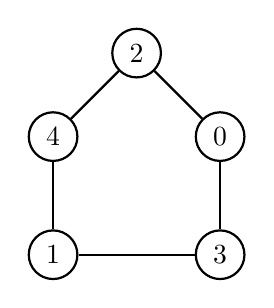
\begin{tikzpicture}[node distance={15mm}, thick, main/.style = {draw, circle}] 
    \node[main] (2) {$2$}; 
    \node[main] (4) [below left of=2] {$4$};
    \node[main] (0) [below right of=2] {$0$};
    \node[main] (1) [below of=4] {$1$};
    \node[main] (3) [below of=0] {$3$};

    \draw (2) -- (4);
    \draw (2) -- (0);
    \draw (4) -- (1);
    \draw (1) -- (3);
    \draw (3) -- (0);
\end{tikzpicture} 
        \caption{Graph $C_5$}
        \label{fig:c5}
    \end{figure}

    Let our cut be $S = \{ 0,1,4 \}$.

    We cut $4$ edges. Thus $OPT \geq 4$.

    \begin{lemma}
        If $k$ is odd, then it is impossible to cut all the edges of $C_k$ (i.e. cycle on $k$ nodes).
    \end{lemma}

    \begin{proof}
        We can try to do cut all the edges by picking nodes with the following procedure.
        Follow the cycle, alternating nodes to pick; i.e.~we pick one and skip the following, then pick the following and skip the one after, and continue to do so.

        Because the cycle is of odd length, then at the end of the cycle we must pick two adjacent nodes, and the edge that connects these two nodes won't be cut.
    \end{proof}

    Note that this is the same reason why we can't have a perfect matching on an odd cycle.

    So, as a corollary, we get that, in $C_5$, $OPT < \cardinality{E} = 5$.

    Thus $4 \leq OPT < 5 \rightarrow OPT=4$.

    Now that we have the optimal value, let us try to solve the SDP for this graph.
    Consider the following solution. $\forall i \in \{ 0,1, \dots, 4 \}$, set:
    \[ \underbar{v}_i = (\cos (i \frac{2\pi}{5}), \sin (i \frac{2\pi}{5}), 0,0,0) \]

    For this solution to be feasible we must have that $\forall i \in V, \underbar{v}_i \cdot \underbar{v}_i = 1$.
    Before showing it, recall that $\forall x, \cos^2 x + \sin^2 x = 1$.

    %$\underbar{v}_i \cdot \underbar{v}_i =
    %\norm{\underbar{v}_i}_2^2 = 
    %\sum_{j=1}^{5} \underbar{v}_i(j) \cdot \underbar{v}_i(j) = 
    %\sum_{j=1}^{2} \underbar{v}_i(j) \cdot \underbar{v}_i(j) = 
    %\cos^2(i \frac{2\pi}{5}) + \sin^2(i \frac{2\pi}{5}) =
    %1$.

    \begin{equation*}
        \begin{split}
            \underbar{v}_i \cdot \underbar{v}_i &= \norm{\underbar{v}_i}_2^2 =\\
                &= \sum_{j=1}^{5} \underbar{v}_i(j) \cdot \underbar{v}_i(j) = \sum_{j=1}^{2} \underbar{v}_i(j) \cdot \underbar{v}_i(j) =\\
                &= \cos^2(i \frac{2\pi}{5}) + \sin^2(i \frac{2\pi}{5}) = 1
        \end{split}
    \end{equation*}

    Thus the solution is feasible.
    Let us now calculate the value of such solution.

    %$SDP =
    %\sum_{\{i,j\} \in E} \frac{1 - \underbar{v}_i \cdot \underbar{v}_i}{2} = 
    %\frac{1 - \underbar{v}_0 \cdot \underbar{v}_2}{2} + \frac{1 - \underbar{v}_2 \cdot \underbar{v}_4}{2} + \frac{1 - \underbar{v}_4 \cdot \underbar{v}_1}{2} + \frac{1 - \underbar{v}_1 \cdot \underbar{v}_3}{2} + \frac{1 - \underbar{v}_3 \cdot \underbar{v}_0}{2} = 
    %\dfrac{1 - \cos(\theta_{02}) + 1 - \cos(\theta_{24}) + 1 - \cos(\theta_{41}) + 1 - \cos(\theta_{13}) + 1 - \cos(\theta_{30})}{2} = 
    %\frac{1 - \cos(\frac{4\pi}{5}) 5}{2} =
    %\frac{5}{2} (1 - \cos (\frac{4\pi}{5})) \approx
    %4.522\dots$

    \begin{equation*}
        \begin{split}
            SDP &=\\
                &= \sum_{\{i,j\} \in E} \frac{1 - \underbar{v}_i \cdot \underbar{v}_i}{2} =\\
                &= \frac{1 - \underbar{v}_0 \cdot \underbar{v}_2}{2} + \frac{1 - \underbar{v}_2 \cdot \underbar{v}_4}{2} + \frac{1 - \underbar{v}_4 \cdot \underbar{v}_1}{2} + \frac{1 - \underbar{v}_1 \cdot \underbar{v}_3}{2} + \frac{1 - \underbar{v}_3 \cdot \underbar{v}_0}{2} =\\
                &= \dfrac{1 - \cos(\theta_{02}) + 1 - \cos(\theta_{24}) + 1 - \cos(\theta_{41}) + 1 - \cos(\theta_{13}) + 1 - \cos(\theta_{30})}{2} =\\
                &= \frac{1 - \cos(\frac{4\pi}{5}) 5}{2} = \frac{5}{2} (1 - \cos (\frac{4\pi}{5})) \approx 4.522\dots
        \end{split}
    \end{equation*}

    Thus, the IG is no better than
    \[ 0.878\dots = \alpha_{GW} \overset{\forall G}{\leq} IG \overset{\exists G}{\leq} \dfrac{4}{4.522\dots} = 0.884\dots \]

    The first inequality (i.e.~$\alpha_{GW} \leq IG$) is actually tight, but tightness is harder to prove.

    So, for Max-Cut we have a $0.878\dots$ approximation that cannot be improved by modifying the random rounding algorithm.
    Can the approximation be improved at all?
    There are reasons to believe that $0.878\dots$ is the best one we can obtain in polynomial time.
